\documentclass[a4paper,12pt,final,oneside,openright]{article}
\usepackage{report}

\newcommand{\reporttitle}{Search Engines and Information Retrieval Systems}
\newcommand{\enseignants}{
Johan Boye\\
Hedvig Kjellström
}

\newcommand{\reportauthor}{
Rémi Domingues}
% \newcommand{\hexanome}{H4211}
\newcommand{\reportsubject}{}
\newcommand{\stagetopic}{Assignment 1 - Boolean retrieval}
\newcommand{\dateperiod}{January $20^{th}$ - February $10^{th}$}
\newcommand{\HRule}{\rule{\linewidth}{0.5mm}}
\setlength{\parskip}{1ex} % Espace entre les paragraphes

\hypersetup{
    pdftitle={\reporttitle},%
    pdfauthor={\reportauthor},%
    pdfsubject={\reportsubject},%
    pdfkeywords={}
}

\title{\reporttitle}
\author{\reportauthor}

\setlongtables
\usepackage[font=small,skip=0pt]{caption}
\usepackage{algorithm}
\usepackage{algpseudocode}


%\setcounter{tocdepth}{4}
\begin{document}
    \renewcommand{\chaptername}{} %\renewcommand{\thechapter}{}
    \renewcommand{\contentsname}{Contents}

    \pagestyle{empty}
    \pagenumbering{arabic}
    % Inspiré de http://en.wikibooks.org/wiki/LaTeX/Title_Creation
\begin{center}
	\begin{minipage}[t]{0.48\textwidth}
	  \begin{flushleft}
	    
\includegraphics [width=30mm]{img/logo_kth.jpg} \\[0.1cm]
		Kungliga Tekniska Högskolan\\
		Valhallavägen 79\\
		100 44 Stockholm
	  \end{flushleft}
	\end{minipage}
	\begin{minipage}[t]{0.48\textwidth}
	  \begin{flushright}
	  \end{flushright}
	\end{minipage} \\[1cm]

	\textsc{\Large \reportsubject}\\[0.3cm]
	\HRule \\[0.4cm]
	{\Huge \bfseries \reporttitle}\\[0.3cm]
	{\LARGE \bfseries «~\stagetopic~»}\\[0.3cm]
	{\Large \dateperiod}\\[0.4cm]
	\HRule \\[1.5cm]

	
\includegraphics [width=0.4\linewidth]{img/icon.png} \\[1.5cm]
	\begin{minipage}[t]{0.5\textwidth}
	  \begin{flushleft} \large
	    \emph{Author}\\
	    \reportauthor
	  \end{flushleft}
	\end{minipage}
	\begin{minipage}[t]{0.4\textwidth}
	  \begin{flushright} \large
	    \emph{Teachers} \\
	    \enseignants
	  \end{flushright}
	\end{minipage}

	\vfill
	\footnotesize{Scholar year 2014-2015}
\end{center}

    \pagebreak
    \sloppy          % Justification moins stricte : des mots ne dépasseront pas des paragraphes

    %\frontmatter
    \thispagestyle{empty}
    %\tableofcontents
    \addtocontents{toc}{\protect\thispagestyle{empty}}
    \pagebreak

    %\mainmatter
    \pagestyle{headings}
    %\renewcommand{\chaptermark}[1]{\markboth{\MakeUppercase{\chaptername\ \thechapter.\ #1}}{}}
    %\renewcommand{\sectionmark}[1]{\markright{\thesection{} #1}}

    \setcounter{section}{3}

\subsection{Relevance feedback}

After having processed a ranked query, our demonstrator gives the user the possibility to select the most relevant results in order to update the query vector as follow to get more accurate results (i.e. more relevant documents):

\begin{equation}
\vec{q} = \alpha \vec{q_0} + \beta \frac{1}{|D_r|} \sum\limits_{\vec{d_j} \in D_r} \vec{d_j}
\end{equation}

The document vector $d_j$ has a sparse representation containing, for each word contained by the document, its frequency (number of occurrences divided by the document length).

$D_r$ is the number of relevant document in the 10 first retrieved documents.

This formule is extracted from the Rocchio's algorithm. Since we only get positive feedback, it is equivalent to the original formula with $\gamma = 0$. \\

\textit{What happens to the two documents that you selected?}

The two selected documents are now higher ranked, since the query perfectly matches their content. This shows that Rocchio's algorithm is working.\\

\textit{What are the characteristics of the other documents in the new top ten list - what are they about? Are there any new ones that were not among the top ten before?}

The results are really different that the previous ones. New documents have been inserted in the top ten and most of them talk about a similar subject than the documents marked as relevant. This should improve the recall of our queries.\\

\textit{How is the relevance feedback process affected by $\alpha$ and $\beta$?}

The higher $\alpha$ is comparing to $\beta$, the more are important the query terms. Otherwise, if $\beta$ is large enough, the most important terms will be the terms occurring the maximal number of times when taking into account every document. Those are likely to be stop words like \textit{a}, \textit{the}, \textit{and}, \textit{or}, which is why $\beta$ must be larger if those terms are not removed.\\

\textit{Why is the search after feedback slower? Why is the number of returned documents larger? Why are there more highly ranked short documents?}

The query has been expanded to take into account the terms of every document selected as relevant. Therefore, the number of matching documents is far higher, and so is the computation time. Short documents are more likely to have a high percentage of terms belonging to the query that long documents, which is why they have a higher TF-IDF score (lower doc length normalization factor)


\subsection{Designing an evaluation}
In order to evaluate the current search engine, we aim at measuring how recall and precision measurements evolve through the Rocchio's algorithm.

\begin{enumerate}
\item Execute the queries \textbf{zombie attack}, \textbf{money transfer} and \textbf{sleeping on campus}
\item Repeat T times
\begin{enumerate}
    \item Let's assume the number of relevant documents is 10. Measure the precision for the following recalls for each query: 0.2, 0.4, 0.6, 0.8, 1
    \item Select the N most relevant documents from the top ten and restart the search
\end{enumerate}
\item Plot T precision-recall curves, the data contained by those plots is the average of the precision for each recall. The search engine should perform well if the area under the curve increase when t increases (i.e. more relevant documents are observed for the same number of retrieved documents).
\item You can also plot, for each query (curve), its precision at 10 for each t. The curves should increase for each query.
\item Eventually, a measure of how well the feedback improves the results could be the average precision at 10 at $t_1$ divided by the same at $t_0$.
\end{enumerate}


\subsection{Speeding up the search engine}
\subsubsection{Index Elimination – use only multi-term occurrences at query time (N terms or more from the query must appear in the document in order for it to be returned)}
This index elimination has been achieved by computing a HashMap containing a document ID as key and the number of query terms contained by the document as value.
When computing the documents TF-IDF vectors, a document which does not satisfy thethreshold requirement is therefore ignored.

\begin{figure}[H]
\centering
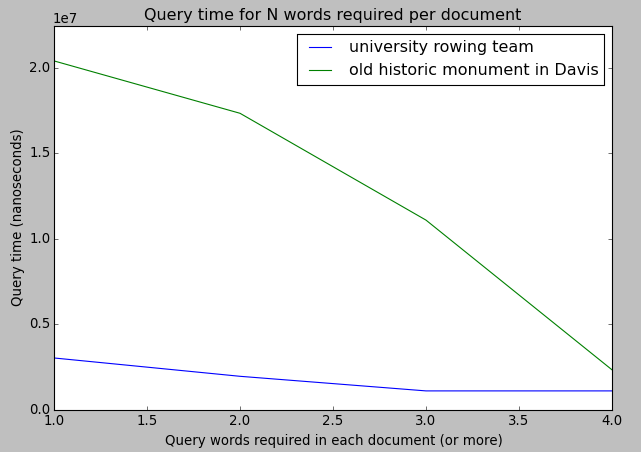
\includegraphics[width=0.7\linewidth]{img/index_elimination_speedup.png}
\end{figure}

\begin{figure}[H]
\centering
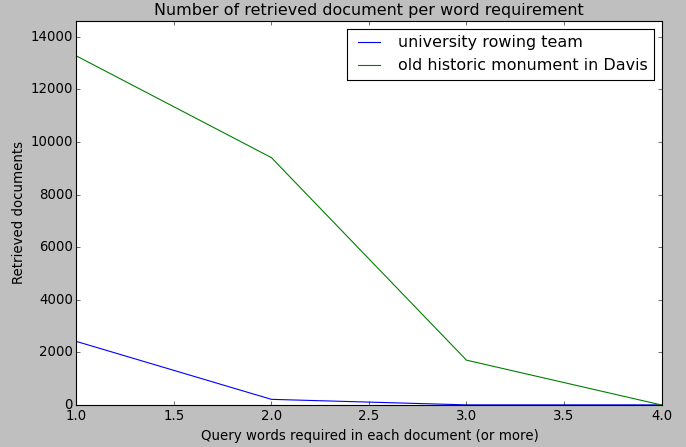
\includegraphics[width=0.7\linewidth]{img/index_elimination_results.png}
\end{figure}

The speed up for 2 words is 1.54 for the first query and 1.17 for the second query.

We can observe that, despite an additional computation time required to process the data structure, an interesting speedup is induced by this index elimination. The speedup is highly correlated to the number of documents satisfying the request.

\subsubsection{Champion Lists - at indexing time, save a list of the N top ranked documents for each term, and use for ranked retrieval}
Since we already computed every TF-IDF score at indexing time (in order to avoid computing the TF-IDF norm of a document at each query for normalization), we know also store the N highest TF-IDF scores and corresponding document for each word.

The champion lists have been obtained by storing in a HashMap the N top-ranked documents for each word. Those documents have been obtained by sorting an array containing pairs of document and TF-IDF score related to a word.

Please note that the following benchmarks have been obtained without the index elimination speed up.

\begin{figure}[H]
\centering
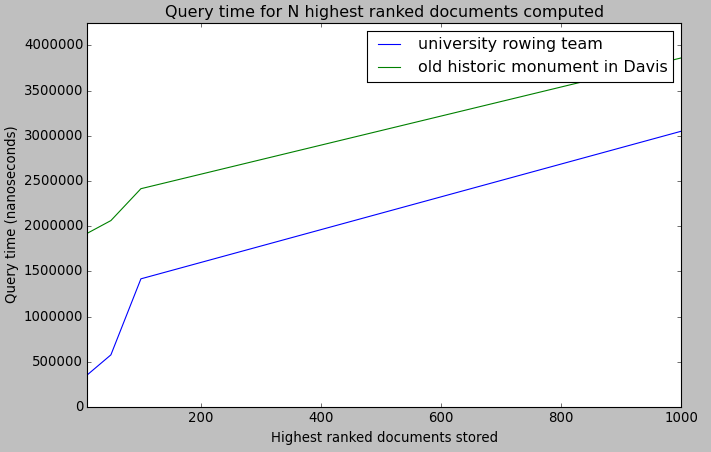
\includegraphics[width=0.7\linewidth]{img/champion_lists_speedup.png}
\end{figure}

\begin{figure}[H]
\centering 
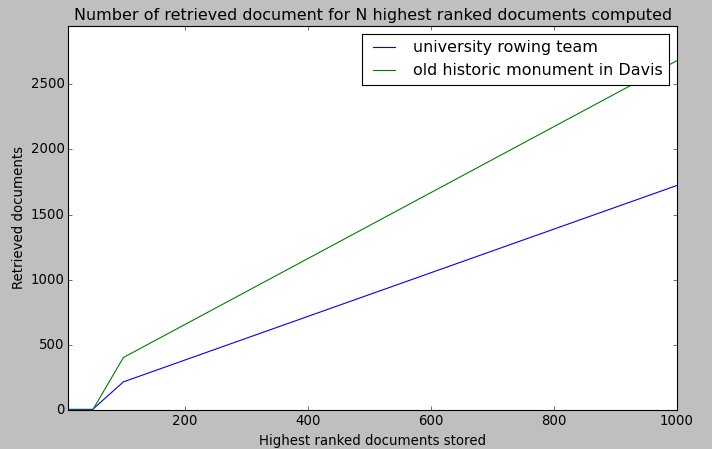
\includegraphics[width=0.7\linewidth]{img/champion_lists_results.png}
\end{figure}

The speed up for 100 documents is 2.14 for the first query and 8.44 for the second query (since \textit{in} probably have many documents).

We should remind here that the query \textit{university rowing team} originally returned 2417 results for a computation time of 3039700 nanoseconds, while \textit{old historic monument in Davis} returned 13272 documents in 20393893 nanoseconds.

Obviously, a delay is observed when indexing, but this is a minor issue since indexing is only processed once and the delay is quite small comparing to the global indexing time (around 5\%).


\subsection{Ranked bigram Retrieval}
The bigram retrieval has been achieved by implementing the class BigramIndex. Is content is similar to HashedIndex, but it can only manage ranked bigram requests.

The data structure used is a HashMap of HashMap, therefore a dictionary containing, for each word, another dictionary (the successor). The value is a postings list containing the occurrences for each document. 

The TF-IDF ranking of a document is then computed like we would for a standard unigram request.

\begin{equation}
tf\_idf_{d,t} = \frac{tf_{d,t}}{len_d} * idf_t
\end{equation}

\begin{equation}
idf_t = log_{10}(\frac{N}{df_t})
\end{equation}

Normalization:

\begin{equation}
\vec{d} = \frac{\vec{d}}{\|\vec{d}\|_{L2}} = \frac{\vec{d}}{\sqrt{\sum{d_i^2}}}
\end{equation}

Cosine similarity:

\begin{equation}
cos(\vec{q}, \vec{d}) = \vec{q} \cdot \vec{d} = \sum{q_i d_i}
\end{equation}


\textbf{zombie attack}

\begin{verbatim}
Found 14 matching document(s)

 0. .\davisWiki\Kearney_Hall.f   0,01890
 1. .\davisWiki\Measure_Z.f   0,01471
 2. .\davisWiki\Spirit_Halloween.f   0,00859
 3. .\davisWiki\Disasters.f   0,00804
 4. .\davisWiki\Biological_Disasters.f   0,00696
 5. .\davisWiki\Scream.f   0,00593
 6. .\davisWiki\Zombie_Walk.f   0,00317
 7. .\davisWiki\Lame_pages.f   0,00278
 8. .\davisWiki\Zombie_Attack_Response_Guide.f   0,00239
 9. .\davisWiki\Explore.f   0,00222
\end{verbatim}

\begin{figure}[H]
\centering 
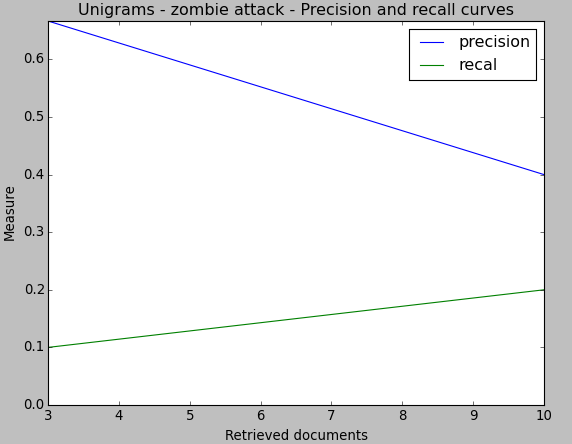
\includegraphics[width=0.7\linewidth]{img/unigrams1.png}
\end{figure}

\begin{figure}[H]
\centering 
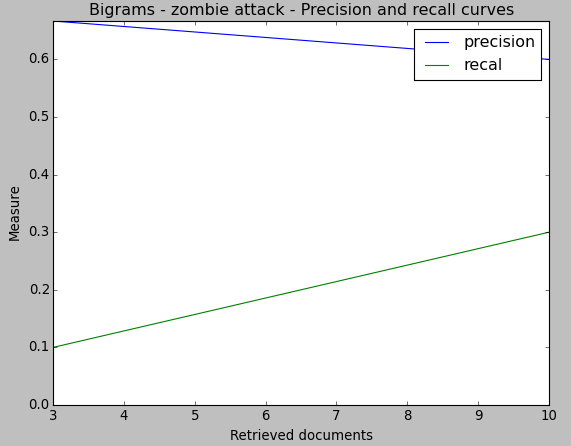
\includegraphics[width=0.7\linewidth]{img/bigrams1.png}
\end{figure}

\textbf{money transfer}

\begin{verbatim}
Found 2 matching document(s)

 0. .\davisWiki\Wells_Fargo_Controversy.f   0,00365
 1. .\davisWiki\Selisa_Romero.f   0,00250
\end{verbatim}

\begin{figure}[H]
\centering 
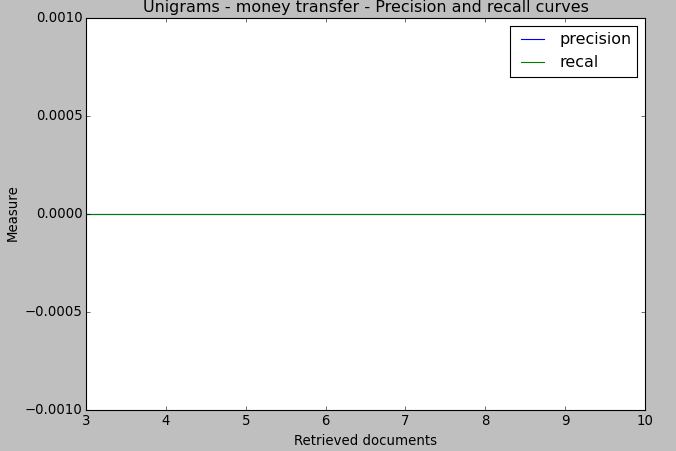
\includegraphics[width=0.7\linewidth]{img/unigrams2.png}
\end{figure}

\begin{figure}[H]
\centering 
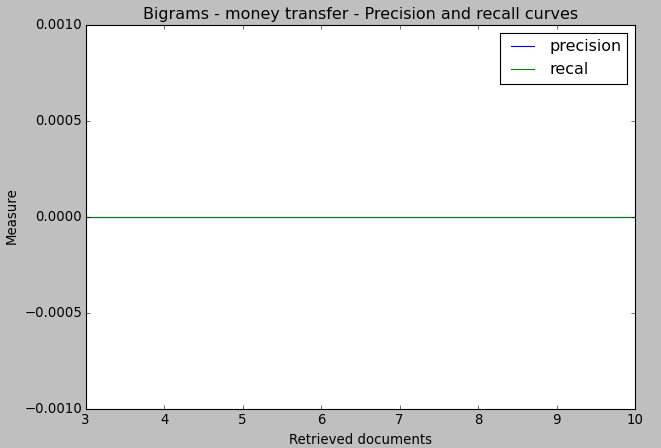
\includegraphics[width=0.7\linewidth]{img/bigrams2.png}
\end{figure}


\textbf{sleeping on campus}

\begin{verbatim}
Found 1202 matching document(s)

 0. .\davisWiki\1934.f   0,03086
 1. .\davisWiki\Chem_Mounds.f   0,03077
 2. .\davisWiki\Smith_Room.f   0,02959
 3. .\davisWiki\Cafe_Fresca.f   0,02429
 4. .\davisWiki\Avian_Sciences_Club.f   0,02419
 5. .\davisWiki\Zinfandel_Lounge.f   0,02128
 6. .\davisWiki\King_Lounge.f   0,01814
 7. .\davisWiki\1969.f   0,01786
 8. .\davisWiki\Hutchison_Trees.f   0,01735
 9. .\davisWiki\Bookhead.f   0,01706
\end{verbatim}

\begin{figure}[H]
\centering 
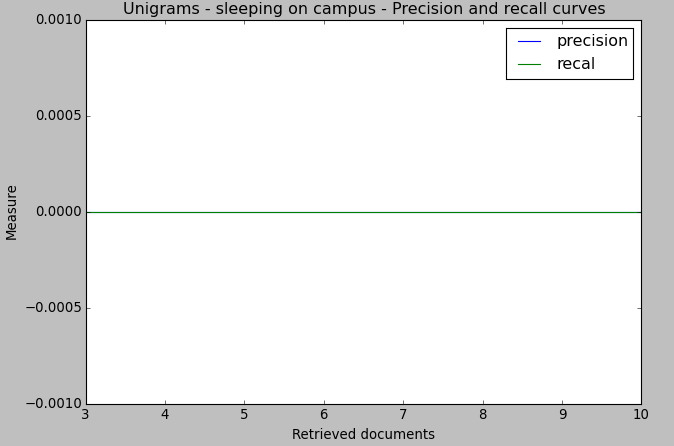
\includegraphics[width=0.7\linewidth]{img/unigrams3.png}
\end{figure}

\begin{figure}[H]
\centering 
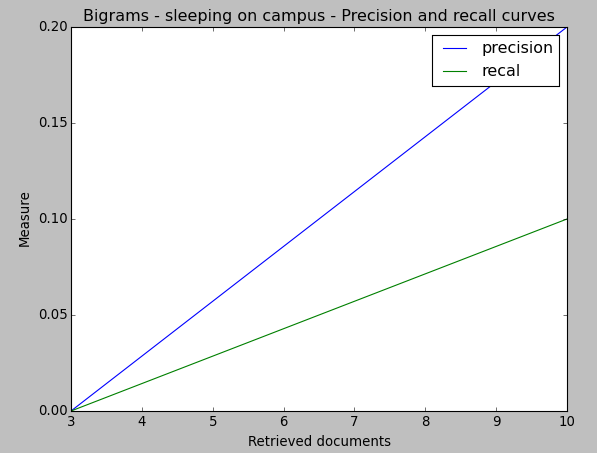
\includegraphics[width=0.7\linewidth]{img/bigrams3.png}
\end{figure}

We obviously have more retrieved documents that with an intersection query but less than with a ranked or union query.

\textit{Are the bigram search results generally more precise than the standard unigram results (higher precision at 3, 10)? Does the bigram ranking list miss important relevant documents, that were returned by the unigram search (lower recall at 3, 10)?}

Given the previous plots for the three queries, bigrams always have a higher or equal precision and recall. The second query is a really hard one since almost no document contain those words one after the other. For the third one, many irrelevant documents are returned due to the term \textit{on}, using bigrams remove those documents. However, the same query still returns very short irrelevant documents for bigrams queries.



    %\backmatter
\end{document}
